\documentclass[12pt]{report}
\usepackage[utf8]{inputenc}
\usepackage[right=2.5cm, left=2.5cm, top=2.5cm, bottom=2cm]{geometry}
%\usepackage{cite}
\usepackage[onehalfspacing]{setspace}
\usepackage{titlesec}
\usepackage{titling}
\setcounter{secnumdepth}{5} % seting level of numbering (default for "report" is 3). With ''-1'' you have non number also for chapters
\setcounter{tocdepth}{5} % if you want all the levels in your table of contents
\usepackage[ngerman]{babel}

%\usepackage[scaled]{helvet}
%\renewcommand{\familydefault}{\sfdefault}

\usepackage{fontspec}

\usepackage{pdfpages}

\titlespacing{\chapter}{0pt}{-49pt}{40pt} %WARUM AUCH IMMER, das zweite Arguments bestimmt den vertikalen Abstand, -49 gibt den richtigen Abstand, verschiebt jedoch auch das Inhaltsverzeichnis nach oben, aber nicht so stark

\titleformat{\chapter}[display]
  {\normalfont\bfseries}{}{0pt}{\Huge} %Das hinten ist das Argument, nutzt "titlesec"
%\titlespacing{<command>}{<left>}{dfdf}{<after-sep>}

%\usepackage{showframe}

\usepackage{packages/sleek-title}
\logo{Abbildungen/logo.png}
\title{Untersuchung der Veränderung des phänologischen Kalenders der Pflanzen im Bezug auf klimatische Unterschiede am Fallbeispiel Jenas}
\institute{Staatliche Gemeinschaftsschule Kaleidoskop Jena}
\faculty{\normalsize Karl-Marx-Allee 11 \\ \normalsize 07747 Jena}
\author{\Large Friedemann Müller \\ Merle Lipowsky \\ Erik Driesch}  
 
\supervisor{\small Seminarfachlehrer: Dr. Clement 
\\      \small Fachbetreuerin: Dr. Krempl 
\\      \small Außenbetreuerin: Dr. Bucher}


\date{Oktober 2023}

\begin{document}

\setmainfont{Arial} %sets main font, who would have guessed

\maketitle
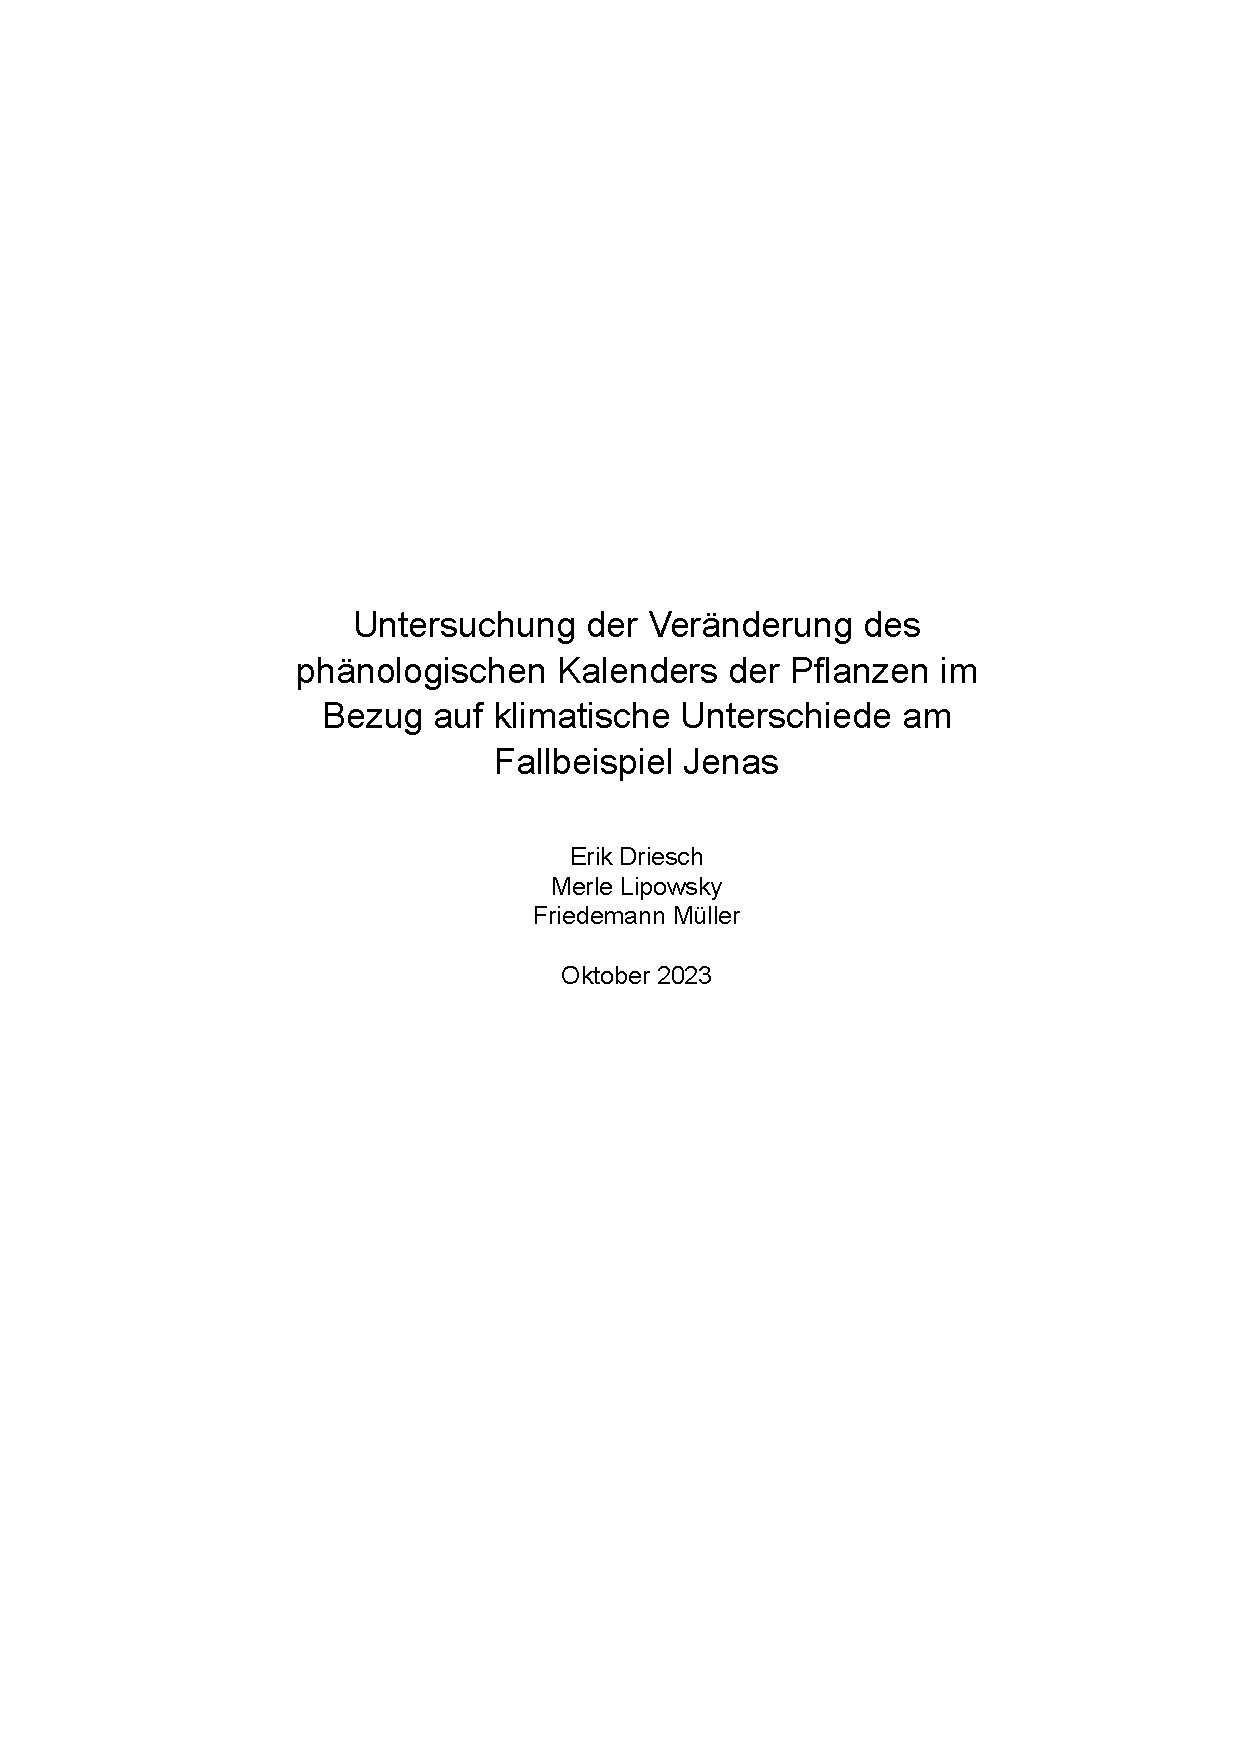
\includepdf[pages=-]{Abbildungen/Titelseite.pdf}
\renewcommand{\contentsname}{Inhaltsverzeichnis}
\tableofcontents
\newpage

\chapter{Abstract}


\chapter{Einleitung}


\section{Warum dieses Thema?}
\section{Hinleitung zur Phänologie}
\section{Thesen}
Unsere Thesen:
\begin{enumerate}
    %\item Der phänologische Kalender besitzt große Relevanz für die landwirtschaftliche Entwicklung.
    

    %\item Der phänologische hat eine große Bedeutung
    %für die historische Entwicklung der Phänologie
    %als Werkzeug für die Landwirtschaft.

    \item Die Nutzung der Pflanzen als zeitliches
    Werkzeug hat der Landwirtschaft erheblichen 
    Vorteile verschafft.
    
    %\item Der phänologische Kalender verändert sich
    %maßgeblich durch den Klimawandel.

    \item Die Veränderung von zeitlich periodischen 
    Entwicklungserscheinungen von Pflanzen beweist 
    die Existenz des Klimawandels. 

    \item (1) Klimatische Unterschiede sind der Grund für die phänologische Differenz zwischen Jenaer Forst und Stadtzentrum.

    \item (2) Klimatische Unterschiede sind der Grund für die phänologische Differenz zwischen urbanen und ruralen Räumen.
    
    %\item Aus klimatischem Unterschied ergibt sich
    %eine phänologische Differenz zwischen Stadt und
    %Land.
\end{enumerate}


\chapter{Theoretische Abhandlung}

\section{Begriffsfestlegungen (Alle geteilt)}
\section{Historik (Friedemann)}
\section{Landwirtschafliche Entwicklung (Friedemann)}
\section{Begründung der Festlegung der Zeigerpflanzen (Merle)}

\chapter{Experiment 1 (Erik und Friedemann)}

\section{Vorüberlegung/Planung (Erik)}
\section{Vorgehen (Erik)} %Wie funktioniert das, wie läuft das ab?
\section{Aufbereitung der Daten (Erik)}
\section{Rückschlüsse aus den Daten / Beantwortung der Thesen (Erik, Friedemann)}
\section{Fehlerbetrachtung}

\chapter{Experiment 2 (Merle, Friedemann)}

\section{Vorüberlegung/Planung (Merle, Friedemann)}
\section{Vorgehen (Merle, Friedemann)}
\section{Aufbereitung der Daten (Merle, Fridemann)}
\section{Rückschlüsse aus den Daten / Beantwortung der Thesen(Merle)}
\section{Fehlerbetrachtung}
\chapter{Zusammenfassung}
\chapter{Anhang}

\section{Datensätze}
\subsection{Datensätze des DWD}
\subsection{Datensätze aus bot. Garten}
\subsection{Datensätze aus dem Forst}

\section{Auswertung in R}

\chapter{Literatur- und Quellenverzeichnis}




\chapter{Eidesstattliche Versicherung}
\noindent
Wir versichern, dass wir die vorgelegte Seminarfacharbeit ohne fremde Hilfe verfasst und keine anderen als die angegebenen Hilfsmittel benutzt haben.
Wir sind damit einverstanden, dass diese Arbeit zu Unterrichtszwecken an den Thüringer Gemeinschaftsschulen Kulturanum und Kaleidoskop verwendet wird.
\newline
\newline
Ort, Datum \qquad \qquad \qquad Unterschrift
\newline
\newline
\newline
Ort, Datum \qquad \qquad \qquad Unterschrift
\newline
\newline
\newline
Ort, Datum \qquad \qquad \qquad Unterschrift 

%\bibliographystyle{plain}
%\bibliography{literatur}
\end{document}
